\chapter{Simple grids} \label{chapter:simple_grids}
In the following we will introduce all kinds of available grids together with their numerical structure. These grids will be the building blocks of the multigrid.
\section{The base class: grid}\index{Grid!class}
As it was shown in chapter \ref{chapter:numerical_integraion} all one needs for numerical integration is the integration grid itself and the corresponding weights. All of this is comprised in the class \texttt{grid} whose members are listed in table \ref{tab:member}. The grid class is defined in the \texttt{grid.h} file as follows

\begin{lstlisting}
class grid
{
        public:
        int M;
        double omega_min;
        double omega_max;
        vector <double> omega;
        vector <double> domega;
        virtual unsigned int inverse (double omega)=0;
};
\end{lstlisting}
The grid itself and its weights are \texttt{vectors} \cite{stl}. The inverse mapping is virtual, and so is the grid class itself. Only the classes which are derived from the grid class are non-virtual. If one is not familiar with the concept of inheritance one can think of it in the following way: Since all integration grids should possess the above attributes (table \ref{tab:member}), it is reasonable to define a skeleton for an integration grid. This is the virtual grid class. It is not possible to create an instance of the grid class, but its possible to give it as an argument in a function. For example:
\begin{lstlisting}
void saveGrid(grid & mgrid, string filename)
{
        ofstream out;
        out.open(filename.c_str());
        for (int j=0; j!=mgrid.M+1; j++)
        {
                out << j << "\t" << mgrid.omega[j] << endl;
        }
        out.close();
}
\end{lstlisting}
This function can then take any kind of grid class (as long as it is derived from the basic grid class) as an argument (for an example, see section \ref{sec:using_the_grid_classes}). This is the whole purpose of using a virtual base grid class. In the following we will introduce all kinds of available grids.

\section{Equidistant grid: equigrid}\label{sec:equigrid}
\index{Grid!equidistant}
\index{equigrid}

The simplest grid class is the equidistant grid class. It is called \texttt{equigrid} and the grid is defined in the following way
\[
	\omega(i) = \omega_{min} + d\omega \cdot i\,,
\]
with $i\in {0,\dots,M}$ and $\omega(M)=\omega_{max}$. Beside the grid class attributes (table \ref{tab:member}), the equigrid has only one additional variable: the grid resolution $d\omega$. The inverse of $\omega(i)$ is given by
\[
	i(\omega)=\frac{\omega-\omega_{min}}{d\omega}
\]
The grid point density reads
\begin{equation}\label{eqn:equigrid_grid_point_density}
 \frac{di}{d\omega} (\omega) = \frac{1}{d\omega}
\end{equation}
The class is defined in the files \texttt{grid.h} and \texttt{grid.cpp}. Its defining member variables are listed in table \ref{tab:equigrid_defining_members}.
\begin{table}[h]
	\begin{center}
		\begin{tabular}{llp{3cm}l}
		Name            & Member                     & Constructor & Description           \\ 
		                &                            & Argument    &                       \\
		\hline
		$M$             & \texttt{int M}             & \nth{1}     & Number of grid points \\
		$\omega_{min}$  & \texttt{double omega\_min} & \nth{2}     & Lower boundary        \\
		$\omega_{max}$  & \texttt{double omega\_max} & \nth{3}     & Upper boundary        \\
		\end{tabular}
	\end{center}
	\caption{Defining properties of the \texttt{equigrid} class}
	\label{tab:equigrid_defining_members}
\end{table}
These are also the arguments of the equigrid constructor which is used for creating an instance of an equigrid:
\begin{lstlisting}
equigrid egrid(M, omega_min, omega_max);
\end{lstlisting}


\section{Tangential grid: tangrid}\label{sec:tangrid}
\index{Grid!tangential}
\index{tangrid}

The tangential grid is called \texttt{tangrid}. Beside the grid class attributes (table \ref{tab:member}), it has a cluster point at $\omega_c$: \\

\begin{center}
	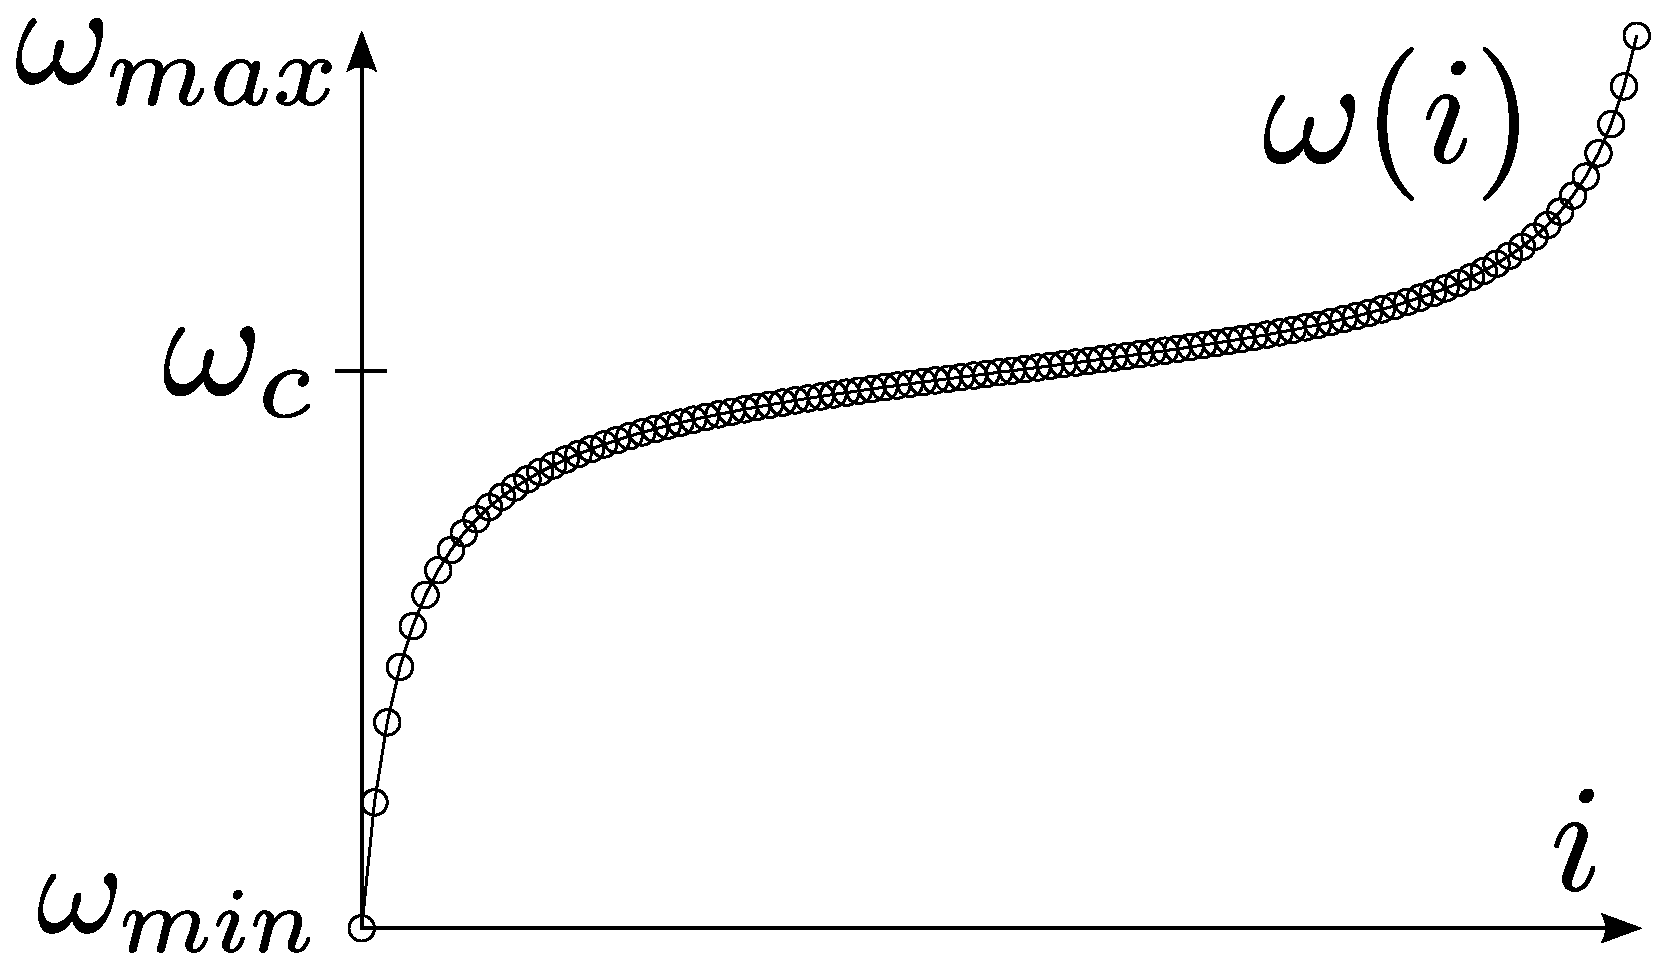
\includegraphics[width=0.3\textwidth]{pics/tangrid.eps}
\end{center}

\noindent The ``sharpness`` of this curve is controlled by the parameter $c$ and the grid is defined by
\[
	\omega(i)= c \tan (u_1+\Delta u \cdot i) + \omega_c
\]
where $i\in \{0,\dots,M\}$, and the parameters $u_1$ and $\Delta u$ are calculated such, that boundary conditions $\omega(0)=\omega_{min}$ and $\omega(M)=\omega_{max}$ are fulfilled. Hence:
\begin{align*}
	u_1&=\arctan\left(\frac{\omega_{min}-\omega_c}{c}\right)\\
	u_2&=\arctan\left(\frac{\omega_{max}-\omega_c}{c}\right)\\
	\Delta u&=\frac{u_2-u_1}{M}
\end{align*}
The inverse of the grid is given by
\[
	i(\omega)=\frac{1}{\Delta u}\left(\arctan\left(\frac{\omega-\omega_c}{c}\right)-u_1\right)
\]
and the point density reads
\begin{equation}\label{eqn:tangrid_grid_point_density}
 \frac{di}{d\omega} (\omega) = \frac{1}{c \Delta u\left(1+\left(\frac{\omega-\omega_c}{c}\right)^2\right)}\,.
\end{equation}

The class is defined in the files \texttt{grid.h} and \texttt{grid.cpp}. Its defining member variables are listed in table \ref{tab:tangrid_defining_members}.
\begin{table}[h]
	\begin{center}
		\begin{tabular}{llll}
		Name            & Member                     & Constructor & Description           \\ 
		                &                            & Argument    &                       \\ 
		\hline
		$M$             & \texttt{int M}             & \nth{1}     & Number of grid points \\
		$\omega_{min}$  & \texttt{double omega\_min} & \nth{2}     & Lower boundary        \\
		$\omega_{max}$  & \texttt{double omega\_max} & \nth{3}     & Upper boundary        \\
		$\omega_{c}$    & \texttt{double omega\_c}   & \nth{4}     & Center point          \\
		$c$             & \texttt{double c}          & \nth{5}     & Controls sharpness   \\
		\end{tabular}
	\end{center}
	\caption{Defining properties of the \texttt{tangrid} class}
	\label{tab:tangrid_defining_members}
\end{table}
These are also the arguments of the tangrid constructor which is used for creating an instance of a tangrid:
\begin{lstlisting}
tangrid tgrid(M, omega_min, omega_max, omega_c, c);
\end{lstlisting}

\section{Logarithmic grid: loggrid}\label{sec:loggrid}
\index{Grid!logarithmic}
\index{loggrid}
To resolve very sharp peaks in the integrand function the logarithmic grid is the right tool. It is named \texttt{loggrid} and it is constructed in the following way. There are three grid regions: one below (I), one around (II) and one above (III) the center point $\omega_k$, which is the point with the highest grid point density.\\

\begin{center}
	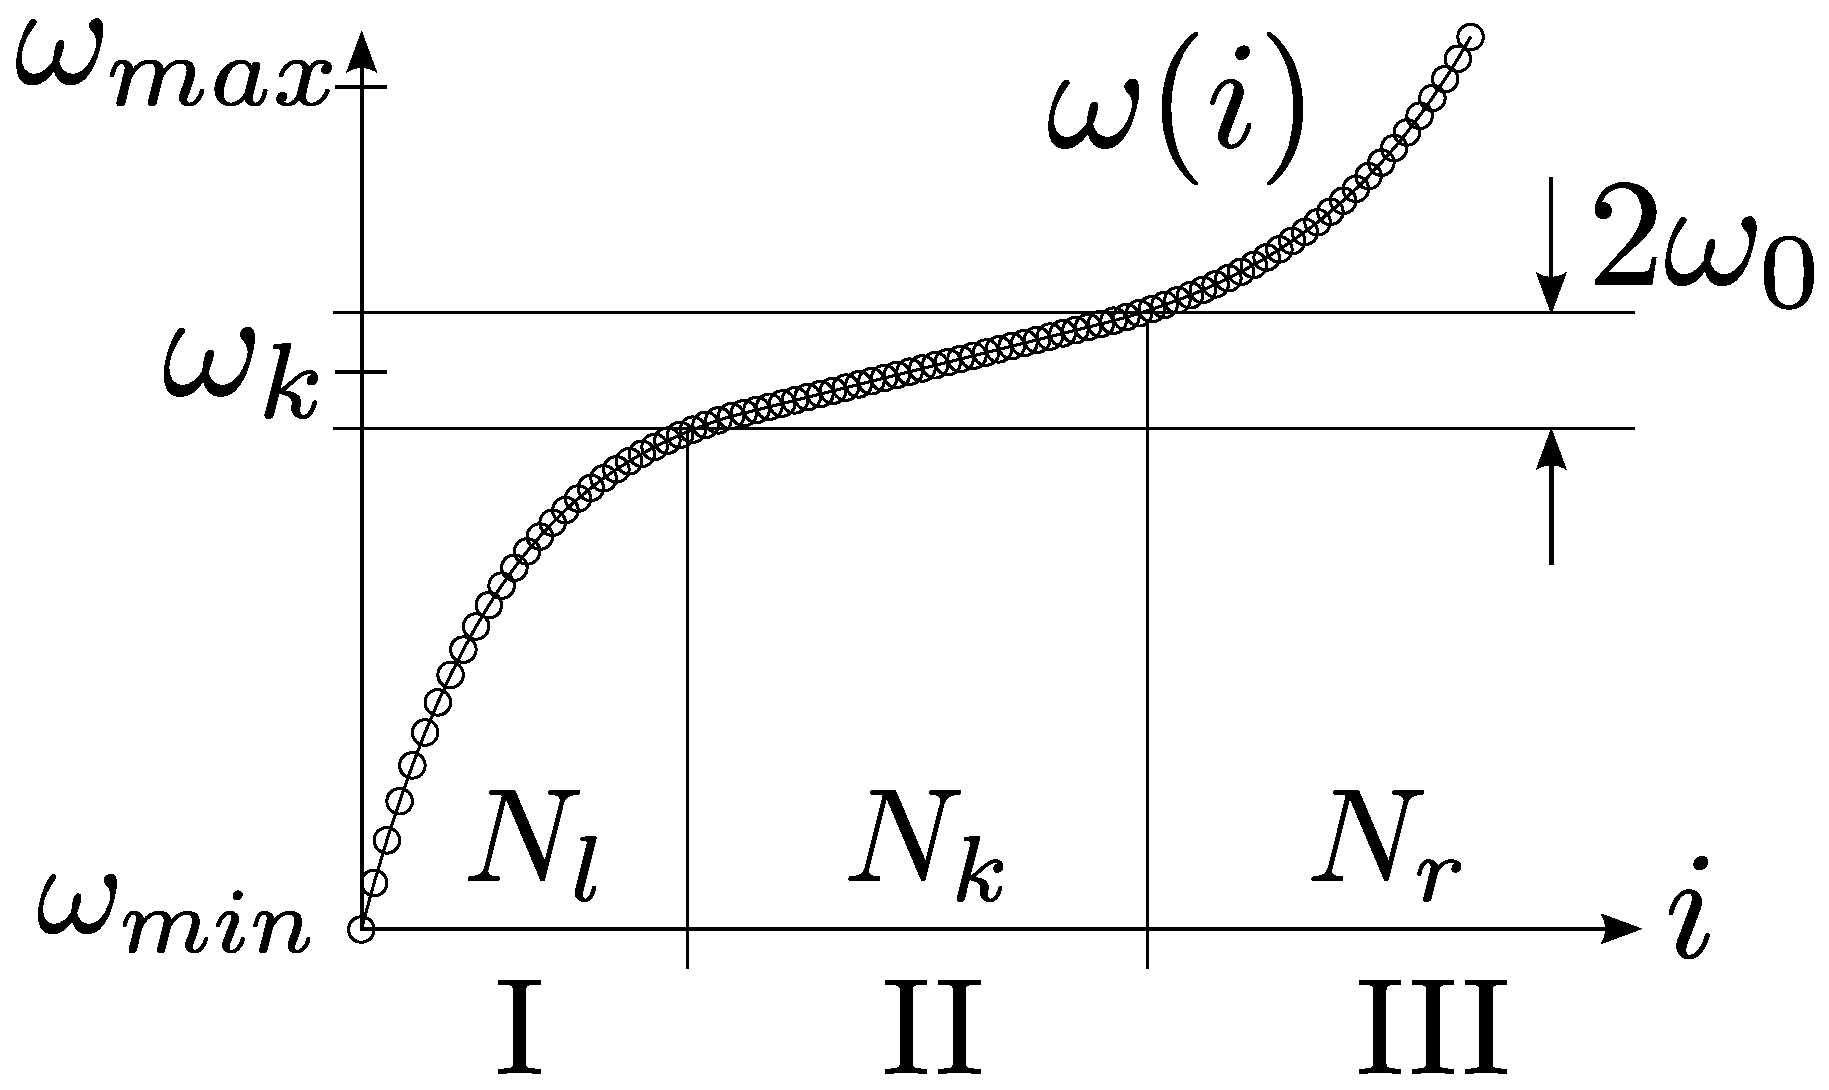
\includegraphics[width=0.4\textwidth]{pics/loggrid.eps}
\end{center}

Region I and III are exponential and region II is linear. The half width of the linear region $\omega_0$ also controls the ''sharpness`` of the exponential grid regions. The number of grid points in region I, $N_l$ and in region III, $N_r+1$ can be chosen different from each other. Both will also influence the ''sharpness'' of the exponential grid regions. The resolution of the linear grid region $d\omega_k$ is the same as the maximal resolution in the exponential grid regions and it determines the number of grid points in region II, $N_k$ (see Appendix \ref{sec:app_loggrid_max_resolution}). The grid is defined as
\begin{equation}\label{eqn:loggrid_definition}
	\omega(i)=\begin{cases}
		-\exp(-c_1(i-i_1)) + \omega_k 		\quad & i\in\{0,\dots,N_l-1\} \\ 
		\omega_k-\omega_0+d\omega_k(i-N_l-1)	\quad & i\in\{N_l,\dots,N_l+N_k-1\} \\ 
		\exp(c_2(i-i_2-N_l-N_k)) + \omega_k 	\quad & i\in\{N_l+N_k,\dots,N_l+N_k+N_r\}
	\end{cases}
\end{equation}
The four boundary conditions
\begin{align}\label{eqn:loggrid_boundary_conditions}
	\omega(0)&=\omega_{min} \quad &\omega(N_l-1)&=\omega_k-\omega_0 \notag \\
	\omega(N_l+N_k)&=\omega_k+\omega_0 \quad &\omega(N_l+N_k+N_r)&=\omega_{max}
\end{align}
determine the four parameters $i_1$, $i_2$, $c_1$ and $c_2$ (see Appendix \ref{sec:app_loggrid_boundary}). The inverse is given by
\[
	i(\omega)=\begin{cases}
		\frac{\log(\omega_k-\omega)}{-c_1} + i_1 \quad &\text{for } \omega\in[\omega_{min},\omega_k-\omega_0] \\
		\frac{\omega-\omega_k+\omega_0}{d\omega_k} + N_l -1\quad &\text{for } \omega\in(\omega_k-\omega_0,\omega_k+\omega_0) \\
		\frac{\log(\omega-\omega_k)}{c_2} + i_2 + N_l + N_k \quad &\text{for } \omega\in[\omega_k+\omega_0, \omega_{max}]
	\end{cases}
\]
and the grid point density reads
\begin{equation}\label{eqn:loggrid_grid_point_density}
	\frac{di(\omega)}{d\omega}=\begin{cases}
		\frac{1}{c_1(\omega_k-\omega)} \quad &\text{for } \omega\in[\omega_{min},\omega_k-\omega_0) \\
		\frac{1}{d\omega_k} \quad &\text{for } \omega\in[\omega_k-\omega_0,\omega_k+\omega_0) \\
		\frac{1}{c_2(\omega-\omega_k)}  \quad &\text{for } \omega\in[\omega_k+\omega_0, \omega_{max}]
	\end{cases}
\end{equation}

The class is defined in the files \texttt{grid.h} and \texttt{grid.cpp}. Its defining member variables are listed in table \ref{tab:loggrid_defining_members}.
\begin{table}[h]
	\begin{center}
		\begin{tabular}{llll}
		Name            & Member                     & Constructor          & Description                         \\ 
		                &                            & Argument             &                                     \\ 
		\hline
		$N_l$           & \texttt{int N\_l}          & \nth{1}              & Number of grid points in region I   \\
		$N_r$           & \texttt{int N\_r}          & \nth{2}              & Number of grid points in region III \\
		$\omega_{min}$  & \texttt{double omega\_min} & \nth{3}              & Lower boundary                      \\
		$\omega_{max}$  & \texttt{double omega\_max} & \nth{4}              & Upper boundary                      \\
		$\omega_{k}$    & \texttt{double omega\_k}   & \nth{5}              & Center point                        \\
		$\omega_{0}$    & \texttt{double omega\_0}   & \nth{6}              & Half width of the region II         \\
		\end{tabular}
	\end{center}
	\caption{Defining properties of the \texttt{loggrid} class}
	\label{tab:loggrid_defining_members}
\end{table}
These are also the arguments of the loggrid constructor which is used for creating an instance of a loggrid:
\begin{lstlisting}
loggrid loggrid(N_l, N_r, omega_min, omega_max, omega_k, omega_0);
\end{lstlisting}

\section{Using the grid classes}\label{sec:using_the_grid_classes}
\index{equigrid}
\index{tangrid}
\index{loggrid}

All of the above grids are derived from the base class \texttt{grid}. Therefore it is possible to write a function which performs the numerical integration without specifying the type of grid one wants to use
\begin{lstlisting}
double integrate(double (&f)(double), grid & g)
{
	double I=0
	for (int i=0; i<=mgrid.M; i++)
	{
		I+= f(mgrid.omega[i]) * domega[i];
	}
	return I;
} 
\end{lstlisting}
which can then be used for example with an equigrid and a Gauss function
\begin{lstlisting}
double gauss(double x)
{
	return exp(-x*x);
}
int main()
{
        equigrid agrid(100, -4, 4);
        //tangrid agrid(100, -4, 4, 1, 0.5);
        //loggrid agrid(30, 30, -4, 4, 1, 0.4);
        double I=integrate(gauss, agrid);
}
\end{lstlisting}
But one can also change the comments in the code in such a way, that a tangrid or a loggrid is used for the integration of a Gauss function.



